\ifx\wholebook\relax\else
\input{../Common.tex}
\input{../macroes.tex}
\begin{document}
\fi

\newcommand{\dist}[0]{middle\xspace}


\chapter{Variables}\label{ch:variables}\label{cha:variable}

\begin{chapterfigure}
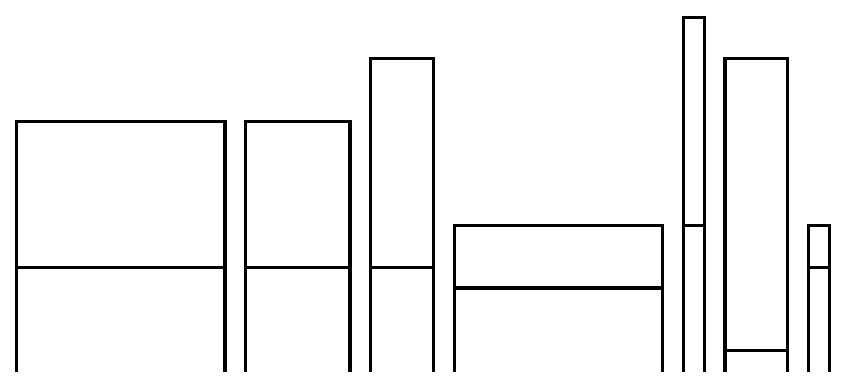
\includegraphics[width=0.9\linewidth]{varTitlePicture}
\end{chapterfigure}

\hidden{|\caro |
	\caro := \Turtle new.
	\caro west.
	\caro jump: 300.
	\caro varALetterHeight: 120 width: 100 middle: 50.
	\caro east.
	
	\caro jump: 10.
	\caro varALetterHeight: 120 width: 50 middle: 50.
	\caro east.
	
	\caro jump: 10.
	\caro varALetterHeight: 150 width: 30 middle: 50.
	\caro east.

	\caro jump: 10.
	\caro varALetterHeight: 70 width: 100 middle: 40.
	\caro east.
	
	\caro jump: 10.
	\caro varALetterHeight: 170 width: 10 middle: 70.
	\caro east.

	\caro jump: 10.
	\caro varALetterHeight: 150 width: 30 middle: 10.
	\caro east.

	\caro jump: 10.
	\caro varALetterHeight: 70 width: 10 middle: 50.


varALetterHeight: height width: width middle: middle


	self north.
	self go: height.
	self east.
	self go: width.
	self south.
	self go: height.

	self west.
	self jump: width.
	self north.
	self go: middle.
	
	self east.
	self go: width.
	self south.
	self go: middle.

}


We are constantly giving names to human beings or things. For example,
we give names to people, to dogs or to cars. By doing that we are
\strong{associating} something to a word or a symbol. Once this association is done,  we \newcommand{\remove}[1]{then} later use the word or symbol to \strong{refer to} or \newcommand{\remove}[1]{to} interact
with the thing associated with it. \newcommand{\replace}[2]{Sometimes,}{Some} names \newcommand{\replace}[2]{are for}{last} a lifetime\newcommand{\replace}[2]{or sometimes}{; others,} just for a short period\newcommand{\remove}[1]{ of time}. \newcommand{\replace}[2]{Sometimes}{Some} names
refer to other names. For example, an actor has several names, a
public name, a civil name and a name of the character he is playing in
a movie. @@dank: that is an example of something having more than one name, but I don't see how it is an example of a name referring to other names.@@  In a programming language\newcommand{\remove}[1]{,} we also need to be able to name things\newcommand{\add}[1]{,} and variables are used for that. 

In this chapter, we introduce \strong{variables} which are \newcommand{\replace}[2]{placeholder}{placeholders} for objects and show  how variables \newcommand{\replace}[2]{helps simplifying}{help simplify} programs. Moreover using variables is sometimes \newcommand{\replace}[2]{mandatory for}{necessary in} programming. So far the scripts you wrote used values (numbers) which, as the complexity of the scripts \newcommand{\replace}[2]{increased}{increase}, are often correlated to each other. In this chapter we show how to use variables to express \newcommand{\replace}[2]{dependencies}{relationships} between
numbers.



\section{A World of As}
As \newcommand{\replace}[2]{asked}{we did} in Chapter~\ref{ch:\newcommand{\replace}[2]{TurtleMen}{turtleMen}}, \newcommand{\replace}[2]{suppose that}{sometimes} we want to use a
robot to write letters. The \newcommand{\add}[1]{shape of the} character A \newcommand{\replace}[2]{is}{can be} characterized by a
\strong{height}, a \strong{width} and a \strong{\dist} \newcommand{\replace}[2]{from which}{--- the distance from the bottom to} the middle line of the A\newcommand{\replace}[2]{ should be drawn}{---} as shown by Figure~\ref{exo:a100}.

\begin{exofigwithsize}{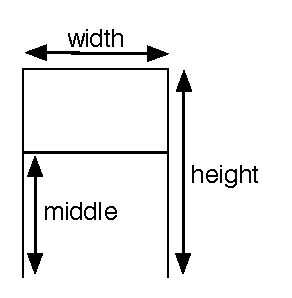
\includegraphics[width=4cm]{varAnnotated}}\label{exo:a100}
Propose a script that draws a character A \newcommand{\add}[1]{with a height} of 100 \newcommand{\replace}[2]{pixel height}{pixels}, \newcommand{\add}[1]{a width of} 70
\newcommand{\replace}[2]{pixel width}{pixels} and \newcommand{\add}[1]{a \dist of} 60 \newcommand{\replace}[2]{pixel \dist}{pixels}.
\end{exofigwithsize}


\paragraph{Variations on A.}
The script you wrote for \newcommand{\remove}[1]{answering the} \exoref{exo:a100} should look
\newcommand{\replace}[2]{somehow}{something} like \newcommand{\replace}[2]{the following script}{Script} \ref{src:a100}.

\begin{scriptwithtitle}{An A \newcommand{\remove}[1]{of} 100\newcommand{\add}[1]{ pixels high}}\label{src:a100}
| \caro |
\caro := \Turtle new.
\caro north.
\caro go: 100.
\caro east.
\caro go: 70.
\caro south.
\caro go: 100.
\caro west.
\caro jump: 70.
\caro north.
\caro go: 60.
\caro east.
\caro go: 70
\end{scriptwithtitle}

\begin{exofigwithsizeandtitle}[0.5]{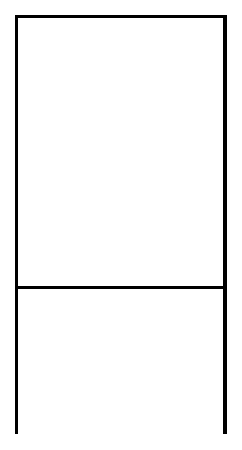
\includegraphics[width=1.5cm]{varA200}}{frAnkenstein}\label{exo:a200}
Change \newcommand{\remove}[1]{the} \scriptref{src:a100} to draw an A \newcommand{\replace}[2]{of}{with} 200 pixel height, 100
pixel width and 70 pixel \dist.
\end{exofigwithsizeandtitle}


As \newcommand{\remove}[1]{the previous} experiment \ref{exo:a200} shows\newcommand{\remove}[1]{ you}, every \newcommand{\replace}[2]{times}{time} we want to produce an A of a different size we have to change \newcommand{\remove}[1]{\strong{everywhere} and
\strong{synchronously}} the numbers that represent the height, the
width and the \dist of the letter\newcommand{\add}[1]{ \strong{everywhere they occur} and \strong{in step with each other}}. By \newcommand{\replace}[2]{synchronously}{in step}, we mean that 100 should \newcommand{\replace}[2]{become}{change to}
200, 70 \newcommand{\add}[1]{to} 100 and 60 \newcommand{\add}[1]{to} 70 \newcommand{\add}[1]{--- all at once, and} without mixing them\newcommand{\add}[1]{ up}.

\begin{exonofig}
Change \newcommand{\remove}[1]{the} \scriptref{src:a100} to draw other \newcommand{\replace}[2]{A letters}{A's} with different
sizes \newcommand{\replace}[2]{of your choice}{you choose}.  Try to reproduce some of the \newcommand{\replace}[2]{As}{A's} \newcommand{\replace}[2]{that compose}{shown in} the opening
picture of this chapter.
\end{exonofig}


As you may notice, having to change the values everywhere is
tedious. Moreover, you \newcommand{\remove}[1]{also may} risk becoming confused and \newcommand{\replace}[2]{forget}{forgetting} to
change a value \newcommand{\replace}[2]{at one place}{someplace}.  This can  result in breaking the
script. You can easily imagine that in complex programs \newcommand{\replace}[2]{this}{it} is
a real problem to change values in \newcommand{\replace}[2]{such a}{this} way.

\section{Variables to the Rescue}
As seen \newcommand{\replace}[2]{with}{in} the previous exercises\newcommand{\add}[1]{,} producing letters of different
\newcommand{\replace}[2]{size}{sizes} is tiresome and \newcommand{\replace}[2]{errorprone}{error-prone}. We have to \newcommand{\replace}[2]{take care}{be careful} to change all
the values everywhere. \newcommand{\replace}[2]{In fact}{Instead}, we would like to be able to:

\begin{itemize}
\item \strong{declare} the height, width and \dist of an A once \newcommand{\add}[1]{and} for all, 
\item \newcommand{\replace}[2]{being}{be} able to \strong{refer to} these values, and 
\item possibly \strong{change} the values if necessary. 
\end{itemize}

This is exactly what a variable allows us to do! Amazing isn't\newcommand{\add}[1]{ it}? A variable is a \strong{name} to which we \strong{associate a value}. We must \emph{declare} it and  \emph{associate} a new value to it. Then we can \strong{refer to} \newcommand{\replace}[2]{a}{the} variable and obtain the \emph{value} associated with \newcommand{\replace}[2]{this variable}{it}. It is also possible to \strong{modify} the value associated with a variable and associate it \newcommand{\add}[1]{with} a new value. The \newcommand{\replace}[2]{variable}{variable's} value can be a number, a collection of objects@@dank: collections haven't been introduced yet, would it be wiser to avoid mentioning them until it's time to define and explain them? Could use Color instead or any other object used earlier in the book.@@, ... even a robot. \newcommand{\add}[1]{\paragraph
}
\newcommand{\replace}[2]{We now}{Next we'll} illustrate how to declare\newcommand{\add}[1]{ a variable}, associate a value and use \newcommand{\replace}[2]{a}{the} variable.

\largecadre{
A variable is a \strong{name} to which we \strong{associate a value}. We \emph{declare} a variable and  \emph{associate} a value to it. Then we can \strong{refer to} \newcommand{\replace}[2]{a}{the} variable and obtain its \emph{value}. It is also possible to \strong{modify} the value associated with a variable and associate a new value to it.}

\subsection*{Declaring a variable}
Before using a variable, we have to \strong{declare} it, \ie \newcommand{\replace}[2]{telling to}{tell} the system the name of the variable that we want to use. We declare variables by enclosing them \newcommand{\replace}[2]{with}{between} vertical bars \ct{||}\newcommand{\replace}[2]{ as shown by the}{. \paragraph

The} following example \newcommand{\remove}[1]{which} declares three variables\newcommand{\add}[1]{:} \ct{height}, \ct{width} and \ct{\dist}.  To be exact, vertical bars \ct{||} declare temporary variables \ie variables that only exist during the execution of the script.

\begin{nalltt}
| height width middle |
\end{nalltt}



\subsection*{Assigning a value to a variable}
Before using a variable it is \newcommand{\replace}[2]{better}{best} to give it a value. Associating a value is called \strong{assigning} a value to a variable. In \st, \ct{:=} is used to assign a value to a variable. In the \newcommand{\replace}[2]{following}{next} script after declaring the three variables we assign 100 to 
the variable \ct{height}, 70 to the variable \ct{width} and 60 to the variable \ct{\dist}.
When \newcommand{\remove}[1]{this is the first time that} we assign a value to a variable\newcommand{\add}[1]{ for the first time}, we say that we \newcommand{\add}[1]{are} \strong{initializing} it.

\begin{nalltt}
| height width middle |
height := 100.
width := 70.
\dist := 60
\end{nalltt}

\largecadre{\ct{:=} assigns a value to a variable. Example: \ct{height := 120} assigns the \newcommand{\add}[1]{number} \ct{120} to the variable \ct{height}.  \ct{length := 120 + 30} assigns the result of the expression  \ct{120 + 30} \ie \ct{150} to the variable \ct{length}.} 

\largecadre{\newcommand{\replace}[2]{When this is the}{The} first time that we assign a value to a variable\newcommand{\add}[1]{,} we say that we \newcommand{\replace}[2]{initialize}{are initializing} it.}

\subsection*{Using Variables}
To use a variable, \ie to refer to the value assigned to it, you
simply write its name in a script. In the \newcommand{\replace}[2]{following}{next} script, after being declared \newcommand{\add}[1]{in} line 1, the variable \ct{height} is initialized  with the value 100 in line 2\newcommand{\replace}[2]{ and}{. Then it is} used \newcommand{\add}[1]{in} line 4 to say to the created robot to go forward \newcommand{\remove}[1]{from} the \ct{height}  variable's value\newcommand{\replace}[2]{, here 100}{ (in this case 100)}.

\begin{nalltt}
| \caro height |
\caro := \Turtle new.
height := 100
\caro north.
\caro go: \textbf{height}
\end{nalltt}

\largecadre{Generally a variable must be \strong{declared} and \strong{initialized}, before being used.}


\subsection*{About \caro}
You guessed right! \caro is also a variable, a variable whose value is a robot. \newcommand{\replace}[2]{Hence,}{So} \ct{| \caro |} declares that we \newcommand{\replace}[2]{use}{have} a variable named \ct{\caro}. The expression \ct{\caro\ := \Turtle new} initializes the variable with a value, here a new robot. Then we use it by sending  it messages, for example \ct{\caro go: 100.}

\section{Using Variables}
Now \newcommand{\replace}[2]{let us}{let's} explore the benefits of using variables and show you some powerful properties. In particular, we show that \newcommand{\replace}[2]{been able}{the ability} to express relationships between variables is really powerful.  

Once we introduce variables in \newcommand{\remove}[1]{the} \scriptref{src:a100}, we \newcommand{\replace}[2]{obtain the}{get}
\scriptref{src:a100var}. Now changing variable values is easier. Change some values to \newcommand{\replace}[2]{convince you}{see for yourself}. \newcommand{\replace}[2]{You should be able to}{Now you can} draw all the As that \newcommand{\replace}[2]{are drawn}{you saw} in the first picture of this chapter.

\begin{scriptwithtitle}{An A \newcommand{\remove}[1]{of} 100\newcommand{\add}[1]{ pixels high}}\label{src:a100var}
| \caro height width \dist|
\caro := \Turtle new.
height := 100.
width := 70.
\dist := 60.
\caro north.
\caro go: height.
\caro east.
\caro go: width.
\caro south.
\caro go: height.
\caro west.
\caro jump: width.
\caro north.
\caro go: dist.
\caro east.
\caro go: width
\end{scriptwithtitle}

\subsection{Expressing Relationships between Variables}
To be \newcommand{\replace}[2]{read efficiently}{easy to read} or simply \newcommand{\add}[1]{to be} nice to look at, a letter should \newcommand{\replace}[2]{respect}{keep}
certain proportions, \ie \newcommand{\replace}[2]{the lengths that describe it}{its measurements} are not
\newcommand{\replace}[2]{freely chosen}{just any numbers} but maintain certain proportions between them. \newcommand{\replace}[2]{Let us}{Suppose we} decide
that the width should be 2/3 of the height and that
the \dist should be \newcommand{\remove}[1]{at} 3/5 of the height. We can express these
relationships using variables\newcommand{\add}[1]{,} as shown in \newcommand{\remove}[1]{the following}
\scriptref{src:a100varl}. \newcommand{\replace}[2]{Indeed the}{The} value of a variable does not have to be 
limited to a simple number but can be the result of a complex computation. 

\begin{scriptwithtitle}{Towards a Solution}\label{src:a100varl}
| \caro height width \dist|
\caro := \Turtle new.
height := \textbf{120}.
width := \textbf{120} * 2 / 3.
\dist := \textbf{120} * 3 / 5.
...
\end{scriptwithtitle}

If you \newcommand{\replace}[2]{analyze a bit the}{think about} \scriptref{src:a100varl}, \newcommand{\replace}[2]{you realize}{you might notice} that it \newcommand{\replace}[2]{is not optimal}{could still be improved}. The relationships are expressed between the variables, but \newcommand{\remove}[1]{still} the value 120 in lines 3,4 and 5 \newcommand{\add}[1]{still} has to be changed manually when we want to produce a different A holding the same \newcommand{\replace}[2]{relations}{proportions}.  \newcommand{\add}[1]{\paragraph
}
The solution is to use the variable \ct{height} instead of \ct{120}\newcommand{\add}[1]{,} as shown in
\newcommand{\remove}[1]{the} \scriptref{src:a100varwl}. In this script, the \newcommand{\replace}[2]{value}{values} of the variables \ct{width} and \ct{\dist} \newcommand{\replace}[2]{depends}{depend} on the \newcommand{\replace}[2]{one}{value} of \ct{height}. As you see
the value of a variable can be expressed by using other variables. 

\begin{scriptwithtitle}{Making \ct{width} and \ct{\dist} \newcommand{\replace}[2]{depending}{depend} on \ct{height}}\label{src:a100varwl}
| \caro height width \dist|
\caro := \Turtle new.
\textbf{height := 120}.
width := \textbf{height} * 2 / 3.
\dist := \textbf{height} * 3 / 5.
\caro north.
...
\end{scriptwithtitle}


\paragraph{Important.} The only \newcommand{\replace}[2]{constraint}{restriction} we have \newcommand{\replace}[2]{while}{when} expressing relationships between variables is that the value of \newcommand{\add}[1]{each} variable used in the definition of
another \newcommand{\replace}[2]{should}{must} be known. For example, in \scriptref{src:a100varwl},
the value of \ct{height} is known while computing the value of
\ct{width} and \ct{\dist}.  \newcommand{\replace}[2]{On the contrary,}{However} in \scriptref{src:wrong} the value of \ct{height} is not known when the value of \ct{width} is computed, \newcommand{\add}[1]{and} this leads to an error. We will \newcommand{\replace}[2]{elaborate}{learn} more \newcommand{\replace}[2]{on}{about} errors in Chapter~\ref{ch:debugger}.

\begin{scriptwithtitle}{Problematic \ct{width} initialization}\label{src:wrong}
| height width \dist |
width := height * 2 / 3.
height := 120.
\dist := height * 3 / 5.
\end{scriptwithtitle}

Now you see that variables are really useful \newcommand{\replace}[2]{to expression}{for expressing} complex relationships\newcommand{\replace}[2]{ and}{. Variables} can hold any kind of objects.

\section{Some \newcommand{\replace}[2]{Experimentations}{Experiments}}
We recommend you gain some experience with the following problems.

\begin{exofigwithsizeandtitle}[.8]{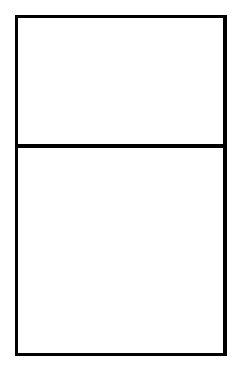
\includegraphics[width=2.5cm]{varGoldenRec}}{Golden Rectangle}\label{exo:goldenrectangle}

A \newcommand{\replace}[2]{golden rectangle}{\strong{golden rectangle}} is a rectangle whose height is 1.6 times its width
--- 1.6 is an approximation of the golden number $\frac{1 +
\sqrt{5}}{2}$\newcommand{\add}[1]{,} which is the side of a regular decagon inside a circle
\newcommand{\replace}[2]{of unity}{with radius 1}.  \newcommand{\replace}[2]{The}{One} nice property of such a rectangle is that if we draw
\newcommand{\remove}[1]{inside the rectangle} a square \newcommand{\replace}[2]{with}{the} size \newcommand{\add}[1]{of} the rectangle's width\newcommand{\add}[1]{ inside the rectangle}, then
the \newcommand{\remove}[1]{left} part of the rectangle \newcommand{\add}[1]{left outside the square} is again a golden rectangle. \newcommand{\replace}[2]{Such a
property is then infinite}{This procedure can be repeated forever}. \newcommand{\add}[1]{\paragraph
}
\newcommand{\replace}[2]{Ancient architects were using a lot such a}{Since ancient times, architects have often used this} golden proportion in their constructions. Every rectangle created this way is a
golden rectangle. \newcommand{\add}[1]{\paragraph
}
Define a script that draws a golden rectangle.
$\frac{1 + \sqrt{5}}{2}$ is expressed in Smalltalk as \ct{1 + 5 sqrt /
2}.

\end{exofigwithsizeandtitle}


\hidden{
| \caro height width|
\caro := \Turtle new.
width := 100.
height := width * ((1 + 5 sqrt)/2).
\caro go: width.
\caro turnLeft: 90.
\caro go: height.
\caro turnLeft: 90.
\caro go: width.
\caro turnLeft: 90.
\caro go: height.
\caro turnLeft: 90.
\caro go: width.
\caro turnLeft: 90.
\caro go: width.
\caro turnLeft: 90.
\caro go: width
}

\begin{exonofig}
Explain why \newcommand{\replace}[2]{none}{neither} of the following scripts \newcommand{\remove}[1]{do not} draw an A \newcommand{\replace}[2]{of}{that is} 120
\newcommand{\replace}[2]{pixel height}{pixels high}.
\begin{nalltt}
\begin{tabbing}
aaaaaaaaaaaaaaaaaaaaaaaaaa\=aaaaaaaaaaaaaaaaaaaaaaaaaa\kill
| \caro height |               \>| \caro height |       \\             
\caro := \Turtle new.         \>\caro := \Turtle new.\\
height := 120.                   \>\caro north.\\
\caro north.                      \>\caro go: height.\\
\caro go: 100.                      \>\caro east.\\
\caro east.                               \>\caro go: 70.\\
\caro go: 70.                               \>\caro south.\\
\caro south.                              \>\caro go: height.\\
\caro go: 100.                             \>\caro west.\\
\caro west.                                 \>\caro jump: 70.\\
\caro jump: 70.                            \>\caro north.\\
\caro north.                                  \>\caro jump: 50.\\
\caro jump: 50.                              \>\caro east.\\
\caro east.                                       \>\caro go: 70\\
\caro go: 70
\end{tabbing}
\end{nalltt}
\end{exonofig}

\paragraph{Pyramids rediscovered.} \newcommand{\replace}[2]{In}{\scriptref{scr:pyramid} in} Section~\ref{sec:bouclonpyramids} of Chapter~\ref{ch:looping} \newcommand{\remove}[1]{in the \scriptref{scr:pyramid} 
we} defined the outline of the pyramid of Saqqarah the following way.

\begin{scriptfigwithsize}[.45]{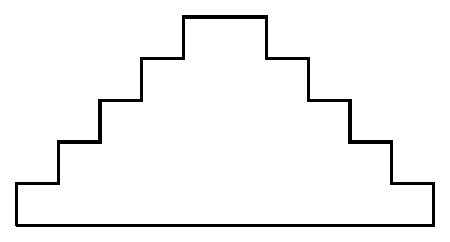
\includegraphics[width=8cm]{varPyramid}}{Pyramid script}
| \caro |
\caro := \Turtle new.
5 timesRepeat: 
               [ \caro north.
               \caro go: 20.
               \caro east.
               \caro go: 20 ].
5 timesRepeat: 
               [ \caro go: 20.
               \caro south.
               \caro go: 20.
               \caro east ].
\caro west.
\caro go: 200.
\end{scriptfigwithsize}


\begin{exonofig}
Introduce the variable \newcommand{\replace}[2]{\ct{terracesNumber}}{\ct{numberOfTerraces}} that represents the
 number of terraces that the pyramid \newcommand{\replace}[2]{can have}{has}. 
\end{exonofig}

\begin{exonofig}
In the previous script introduce the variable \ct{terraceSize} that represents the size of a terrace.
\end{exonofig}
 
\section{Another Example of \newcommand{\replace}[2]{Variable Use}{Using Variables}}
The use of variables greatly simplifies the definition of scripts where some of the \emph{variables} depend on other ones. In this section, we shall see how the use of variables gives great leverage when dealing with loops. \newcommand{\remove}[1]{The} Chapter~\ref{ch:loopvar} will go deeper\newcommand{\replace}[2]{ in}{,} showing that the combination of variables and loops is powerful.

\newcommand{\replace}[2]{Let us}{Let's} look again for a moment at \newcommand{\replace}[2]{the experiements}{experiments} ~\ref{exo:pentagonRepeat} and
\ref{exo:hexagonRepeat}\newcommand{\add}[1]{,} in which a \Turtle was asked to draw a
pentagon and a hexagon. 

\begin{scriptfigwithsize}[.5]{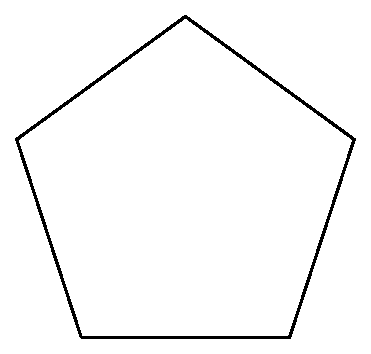
\includegraphics[width=4.5cm]{varFPentagon}}{Pentagon}
| \caro |
\caro := \Turtle new.
5 timesRepeat: 
               [ \caro go: 100.
               \caro turnLeft: 72 ]
\end{scriptfigwithsize}

\begin{scriptfigwithsize}[.5]{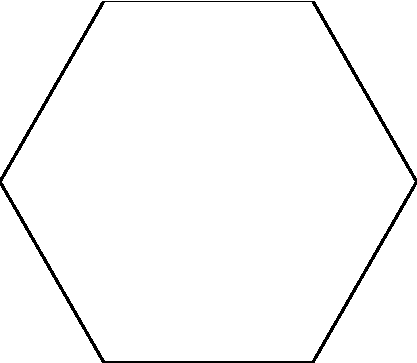
\includegraphics[width=4.5cm]{varFHexagon}}{Hexagon}
| \caro |
\caro := \Turtle new.
6 timesRepeat: 
               [ \caro go: 100.
               \caro turnLeft: 60 ]
\end{scriptfigwithsize}

\newcommand{\replace}[2]{The difference between the two scripts is that}{To change the first script into the second,} one must change the
number of sides (\newcommand{\replace}[2]{let us}{we'll} call \newcommand{\replace}[2]{it $s$}{that $sides$}) \emph{and} the magnitude of the
turn (\newcommand{\replace}[2]{let us}{we'll} call \newcommand{\replace}[2]{it $T$}{that $angle$}) \newcommand{\replace}[2]{such}{so} that the product \newcommand{\replace}[2]{$s\times T$}{$sides$ \times $angle$} is equal
to 360.\newcommand{\add}[1]{\paragraph
}
Wouldn't it be nice if we could write a script\newcommand{\remove}[1]{,} in which we
\newcommand{\remove}[1]{only} would have to change \newcommand{\add}[1]{only} a single number\newcommand{\replace}[2]{,}{ to switch between drawing the pentagon and the hexagon?} \newcommand{\replace}[2]{let us say}{Let's pick} the number of
sides \newcommand{\add}[1]{$sides$ to be that single number,} since \newcommand{\replace}[2]{this}{it} is the easiest parameter to choose\newcommand{\replace}[2]{?}{.}  This is possible
by introducing variables. \newcommand{\add}[1]{\paragraph
}
Try to come up with your own solution.  




Here is a script \newcommand{\replace}[2]{where this is done}{that does it} (Script~\ref{scr:regularPolygon}). Try it
before we discuss \newcommand{\replace}[2]{more about it}{it some more}. 

\begin{scriptwithtitle}{Regular polygon}\label{scr:regularPolygon}
| \caro sides angle |
\caro := \Turtle new.
sides := 6.
angle := 360 / sides.
sides timesRepeat: 
                  [ \caro go: 100.
                  \caro turnLeft: angle ]
\end{scriptwithtitle}

We have introduced two new
variables --- \ct{sides} and \ct{angle} --- used to hold
the needed values. Then\newcommand{\remove}[1]{,} the line \ct{sides := 6} assigns the
value 6 to the variable \ct{sides}\newcommand{\replace}[2]{ and the}{. The} line \ct{angle
:= 360 / sides} assigns a value to the variable angle, \newcommand{\replace}[2]{which is}{namely}
the result of 360 divided by the value held in the variable
\newcommand{\replace}[2]{\ct{number}}{\ct{sides}}. The value of the variable \ct{angle} is then
used as argument of the \newcommand{\remove}[1]{command} \turnLeft \newcommand{\add}[1]{command} given to
the robot in the repeating block.

@@dank: Would it make sense to add a sentence here suggesting the student try it out?  Something like \newcommand{\add}[1]{Try running Script~\ref{scr:regularPolygon} and changing the value of \ct{sides}.}  It seems parallel to your practice for earlier examples.@@

\section{Regular Polygons with Fixed Sizes}

If you \newcommand{\remove}[1]{have} used Script~\ref{scr:regularPolygon} with a large number of sides, you \newcommand{\replace}[2]{will have}{probably} noticed that the resulting figure did not fit on the screen.  The next exercise asks you to fix this by reducing the
length of the sides when the number of sides \newcommand{\replace}[2]{augments}{grows larger}.

\begin{exofig}{varSameLength} \label{exo:fixedSizePolygon}
Modify Script~\ref{scr:regularPolygon} so that the size of the
regular polygon stays constant as the number of sides changes.

Hint: introduce a variable \newcommand{\replace}[2]{length}{\ct{length}} which is set to \newcommand{\replace}[2]{a fixed length}{some constant number}
divided by the number of sides.
\end{exofig}

\hidden{| \caro sides angle l |
	\caro := \Turtle new.
	sides := 15.
	angle := 360 / sides.
	l := 300 / sides.
	sides timesRepeat: [ \caro go: l.
                  \caro turnLeft: angle ]}

\summa

\begin{enumerate}
\item A variable is a \strong{name} to which we \strong{associate a value}. We must \emph{declare} it and  \emph{associate} a value to it. Then we can \strong{refer to} \newcommand{\replace}[2]{a}{the} variable and obtain the \emph{value} associated with \newcommand{\replace}[2]{this variable}{it}. It is also possible to \strong{modify} the value associated with a variable and associate a new value to it. 
 
\item A variable can be used at any place \newcommand{\add}[1]{in a script} where its value \newcommand{\replace}[2]{can}{could} be used.  

\item \newcommand{\replace}[2]{When this is the}{The} first time that we assign a value to a variable, we say that we \newcommand{\replace}[2]{\strong{initialize}}{are \strong{initializing}} it. 

\item \ct{:=} assigns a value to a variable. Example: \ct{height := 120} assigns the \newcommand{\add}[1]{value} \ct{120} to the variable \ct{height}.  \ct{length := 120 + 30} assigns the result of the expression  \ct{120 + 30} \newcommand{\replace}[2]{\ie}{(which is the value} \ct{150}\newcommand{\add}[1]{)} to the variable \ct{length}.

\item A variable must be \strong{declared} and \strong{initialized}, before being used.

\end{enumerate}


\begin{table}[h]
  \centering
\begin{tabular}{| p{5cm} | p{4cm} | l |} \hline
  \hfil Expressions & \hfil Description & \hfil \newcommand{\replace}[2]{Example}{Examples} \\[1ex] \hline
  \ct{| $\langle$variable name$\rangle$ |} & Declaration of \newcommand{\replace}[2]{a variable}{one or more variables} & \ct{| \caro height |}\\ \hline
  \ct{$\langle$length$\rangle$ := $\langle$ \emph{expression} $\rangle$} & Assigns the  value of \newcommand{\replace}[2]{expression}{\ct{expression}} to \newcommand{\replace}[2]{a}{the} variable\newcommand{\add}[1]{ \ct{length} & \ct{length\ :=\ 40}\\
  && \ct{length := 30 + 20}\\ \hline
  &Uses a variable's value& \ct{\caro go: length}\\ \hline

  &Uses and changes the value of a variable& \ct{length := length + 10}\\
  \hline
\end{tabular}
\end{table}


\ifx\wholebook\relax\else\end{document}\fi
